%% LyX 2.0.2 created this file.  For more info, see http://www.lyx.org/.
%% Do not edit unless you really know what you are doing.
\documentclass[12pt,twoside,british,english]{report}
\usepackage{lmodern}
\renewcommand{\familydefault}{\rmdefault}
\usepackage[T1]{fontenc}
\usepackage[latin9]{inputenc}
\usepackage[a4paper]{geometry}
\geometry{verbose,tmargin=3.5cm,bmargin=3cm,lmargin=3.5cm,rmargin=3cm,footskip=1cm}
\usepackage{fancyhdr}
\pagestyle{fancy}
\setcounter{secnumdepth}{3}
\setcounter{tocdepth}{3}
\setlength{\parskip}{\medskipamount}
\setlength{\parindent}{0pt}
\usepackage{float}
\usepackage{textcomp}
\usepackage{amsmath}
\usepackage{amssymb}
\usepackage{graphicx}
\usepackage{setspace}
\usepackage[authoryear]{natbib}
\usepackage{nomencl}
% the following is useful when we have the old nomencl.sty package
\providecommand{\printnomenclature}{\printglossary}
\providecommand{\makenomenclature}{\makeglossary}
\makenomenclature
\setstretch{1.5}

\makeatletter
%%%%%%%%%%%%%%%%%%%%%%%%%%%%%% User specified LaTeX commands.
\usepackage{fancyhdr}
\pagestyle{fancy}
\fancyhead[RE]{\bfseries \nouppercase\leftmark}
\fancyhead[LO]{\bfseries \nouppercase \rightmark}

\renewcommand{\chaptermark}[1]{%
\markboth{\chaptername 
\ \thechapter\ }{}}

 
\fancyhead[LE,RO]{\bfseries\thepage}
\fancyfoot{}
\raggedbottom
\setlength{\parindent}{8mm}

\makeatother

\usepackage{babel}
\begin{document}

\chapter{Covariance of the Wind and Solar Fields \label{chap:Cov-Wind-Solar}}

\newpage{}


\section*{Summary}

\noindent This chapter presents an analysis of the covariance of the
wind and solar fields from the ERA-Interim data set. By \foreignlanguage{british}{utilising}
the continental SOM from \ref{sec:Creating-the-SOM} this chapter
discusses the wind and solar conditions that co-occur with the common
synoptic weather types of the Australian region. Following this, an
in depth analysis of particular weather types that lead to both favourable
and detrimental wind and solar power conditions is undertaken, with
conclusions about how an interconnected renewable electricity based
power system for Australia might be affected by large-scale synoptic
weather phenomena.

\noindent \newpage{}


\section{Introduction and Methods\label{sec:Covariance-Intro-Methods}}

In the current study the decision was made to analyse wind and solar
capacities (instantaneous or average percentage of maximum), rather
than analyse the raw fields, as this was seen as the easiest way to
compare the two variables. Wind and solar capacities were used as
an indicative measure of the likely operating percentage of a renewable
electricity installation at each location without a pre-determination
about the size or type of installation. It should be noted that the
Singular Value Decomposition (SVD) method for simultaneously analysing
the wind and solar fields was examined but not included. SVD is the
two variable extension to Principle Component Analysis and produces
simultaneously co-occurring patterns (spatial patterns and their time
series). However, the ERA-Interim solar irradiance data contained
very limited temporal information beyond the seasonal and diurnal
cycles, which dominate. Thus the results from the SVD investigation
of ERA-Interim data were not included in the thesis.

Wind capacity was calculated by first determining the equivalent power
output. Wind power has a non-linear relationship with wind speed and
in the current study the wind power curve for a General Electric \nomenclature{GE}{General Electric}(GE)
2.5MW turbine (Fig. \ref{fig:GE-2.5-Power-Curve}) was used to convert
wind speed to potential wind power output. GE is the single largest
manufacturer of wind turbines in the world (\citealp{REN212013})
and most of the land-based turbines installed around the world have
a rating of between 1.5 and 3.5MW (\citealp{REN212013}). 
\begin{figure}[H]
\begin{centering}
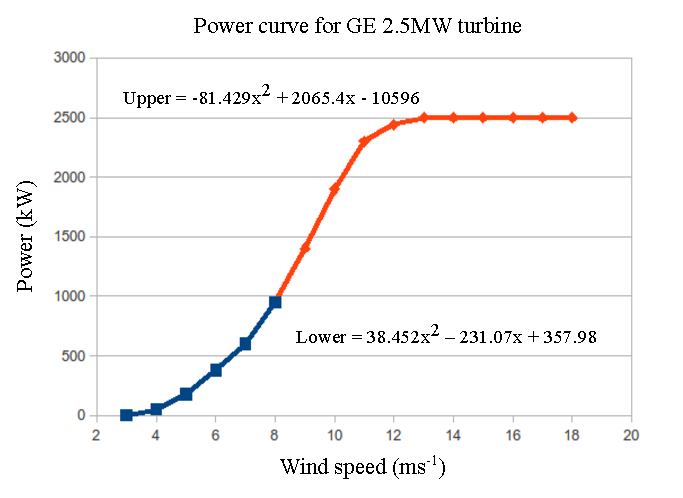
\includegraphics{Figures/Power_curve}
\par\end{centering}

\caption{Data points for a GE 2.5MW wind turbine. Two quadratic fits are used
to approximate the curve where the power output is not 0MW or at the
rated 2.5MW. \label{fig:GE-2.5-Power-Curve}}
\end{figure}


Using the two quadratic curves from Fig. \ref{fig:GE-2.5-Power-Curve},
the moments of no output for wind speeds smaller than 3ms\textsuperscript{-1}
(cut-in) and greater than 18 ms\textsuperscript{-1} (cut-out), and
the rated curve from 12ms\textsuperscript{-1} to 18ms\textsuperscript{-1},
the potential wind power output was calculated for any given wind
speed value. The wind speed values used were interpolated to 80m above
ground using a cubic spline through the first few pressure levels
of the ERA-Interim data. The interpolation was calculated in order
to represent the wind speeds at a standard wind turbine hub-height,
and was necessary due to the typical change in wind speed with height
in the atmosphere. The wind capacity was then a percentage of maximum
(2.5MW) at any one point in time, and the wind capacity factor was
the accumulated power as a percentage of what would have been accumulated
had an installation been running at 100\% for all of the time.

For the current study, solar capacity was not calculated as a percentage
of maximum power output, but as a percentage of maximum Downward Shortwave
Radiation (DSR) levels instead. Maximum irradiance was taken as the
maximum solar irradiance value for all time and space (980 Wm\textsuperscript{-2}
for the accumulation between 2100UTC December 11 1995 and 0300UTC
December 12 1995, and at 151.5�E and 30�S), which was then used as
a proxy for all types of solar power (solar thermal, photo-voltaic,
concentrating solar thermal etc.). It should be noted, however, that
the irradiance data from ERA-Interim are three-hourly accumulated
values. The accumulated values were taken as three hour blocks either
side of each time-step of the analysis fields, and these values were
then averaged. The solar capacity at any one point in time was then
a percentage of 980 Wm\textsuperscript{-2} and the solar capacity
factor was the accumulated irradiance as a percentage of what would
have been accumulated had the irradiance been 980 Wm\textsuperscript{-2}at
all times. It was assumed that any type of solar installation would
have been operating at capacity on December 12 1995 (0000UTC) at 151.5�E
and 30�S, and thus using 980 Wm\textsuperscript{-2} as the measure
of capacity was a useful first guess of solar availability at each
location. 

Further, it was also decided not to convert the DSR data to an equivalent
power output. DSR is the global shortwave radiation falling on a horizontal
plane at surface of the Earth, which would be most closely related
to PhotoVoltaic power output. Indeed it is possible to employ mathematical
models to convert incoming radiation to power output (for instance,
\citet{Villalva2009}), however, it has also been shown over longer
periods of time (yearly, and therefore also longer) to make little
difference (\citet{Perpinan2008}). \citet{Perpinan2008} in their
study of grid connected PV in Spain showed that total PV output for
a year can be approximated, with errors below 3\%, from solar irradiance
values. This thesis is primarily concerned with spatial variance in
the solar resource and less on the strict implementation of solar
power output in an electricity system. While taking into account other
influences on solar power output (in particular temperature on PV)
would be a more accurate description of solar electric output it would
not be a more accurate description of the spatial variance of the
solar potential and how it varies in relation to wind power potential
(as well as the influence of particular synoptic weather types).


\section{Covariance Results and Discussion\label{sec:Cov-Results-and-Discussion}}

Using the time series of SOM node occurrences the wind and solar capacity
factors were calculated for each SOM node and the results are shown
in Fig. \ref{fig:SOM-Bivar-Wind-Solar}. Fig. \ref{fig:SOM-Bivar-Wind-Solar}
illustrates the average wind power and solar capacity factor at each
grid point on the Australian continent when each of the SOM pressure
distributions were said to occur in the 1989-2009 ERA-Interim data.
\begin{figure}[H]
\begin{centering}
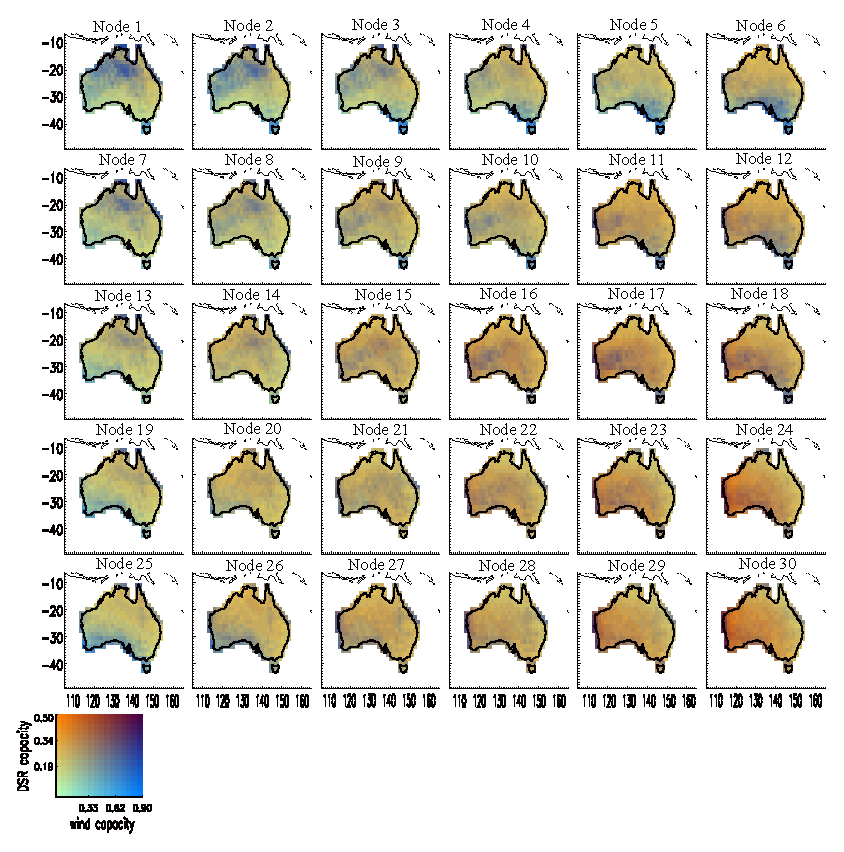
\includegraphics{Figures/average_capacity_per_node-wind_solar_RGB_middle}
\par\end{centering}

\caption{Simultaneous representation of the average capacity of both wind and
solar for each SOM node, from the SOM depicted in Fig. \ref{fig:6x5-SOM-space-Cont}.
Average capacity refers to the average wind power/DSR value at each
location when that SOM node is said to occur, as a percentage of maximum
for each location. Colours are from the colour table, which has an
increasing blue component for larger wind capacities and a larger
red component for increasing DSR capacities\foreignlanguage{british}{---for
instance purple indicates a location with both high average wind and
solar capacity. Colour} scheme adapted from \citet{Teuling2011}.
\label{fig:SOM-Bivar-Wind-Solar}}
\end{figure}


Results from Fig. \ref{fig:SOM-Bivar-Wind-Solar} illustrate that
upon preliminary investigation there were some SOM nodes, or weather
regimes, that appeared to be favourable for both wind and solar capacity
simultaneously. Nodes from the bottom right corner of Fig. \ref{fig:SOM-Bivar-Wind-Solar},
which predominantly occurred in summer, seemed to have both a high
average solar radiation and high average wind power capacity in Western
Australia (WA). During winter months it appeared as if concurrently
higher values of wind and solar capacity were rare. In fact, node
20 from Fig. \ref{fig:SOM-Bivar-Wind-Solar} appears to have low capacity
factors for both wind and solar across virtually the entire Australian
continent. The exception for winter was perhaps northern Australia
during a high in the Bight regime (node one or two from Fig. \ref{fig:6x5-SOM-space-Cont})
where average wind capacity values reached 0.6 and average solar capacity
values reached 0.3. 

Based on Fig. \ref{fig:SOM-Bivar-Wind-Solar}, some important considerations
for the spatial relationship between the wind power and DSR capacities
across the Australian continent (and therefore potentially a renewable
electricity network that encompasses the same area) could be highlighted.
In particular some SOM nodes appeared to be associated with both concurrently
low or high wind and solar capacities. Such nodes included node 20
(low capacity of both wind and solar), node 24 (high capacity of wind
and solar along the coast of WA) and node 18 (higher solar capacity
in the West and higher wind capacities in the South); and thus these
nodes also required a more detailed analysis of the atmospheric conditions
they represent. 

SOM node 20---classified by a high pressure system \foreignlanguage{british}{centred}
just East of Victoria that also ridges across much of the Australian
continent (Fig. \ref{fig:Nodes-of-Interest-MSLP}b)---was largely
characterised by low average wind power and DSR capacities for most
of the Australian continent (Fig. \ref{fig:Node-20-Wind-Dsr-Cap}).
\begin{figure}[H]
\begin{centering}
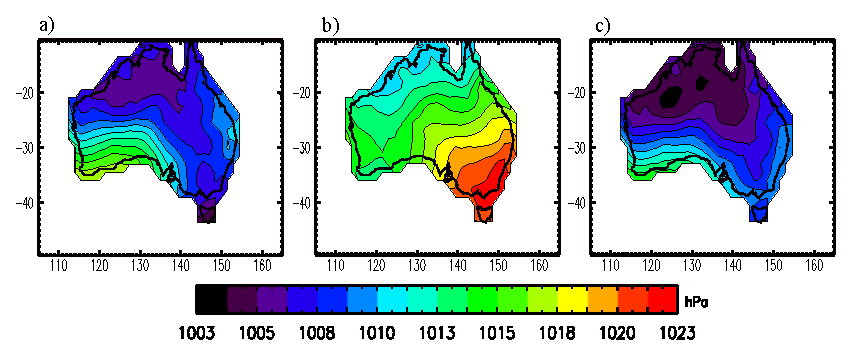
\includegraphics{Figures/Nodes_18_20_24_mslp}
\par\end{centering}

\caption{MSLP maps for continental SOM nodes a) 18, b) 20 and c) 24. Values
in the colourbar have been truncated at the nearest whole number for
readability purposes. \label{fig:Nodes-of-Interest-MSLP}}
\end{figure}
\begin{figure}[H]
\begin{centering}
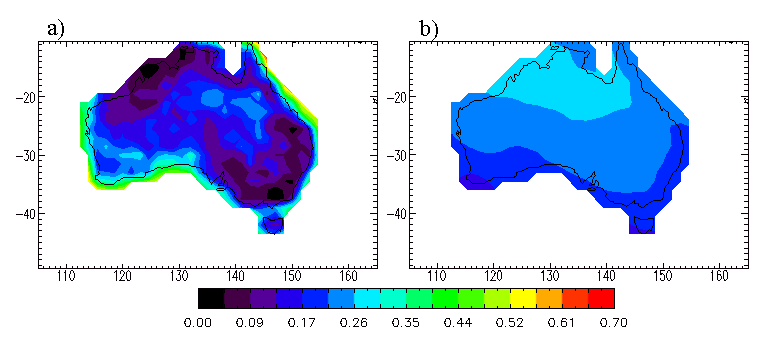
\includegraphics{Figures/Node_20_average_power-cap_wind}
\par\end{centering}

\caption{Average capacity when continental SOM node 20 occurs for a) wind power
and b) DSR. Average capacity for wind and DSR is as defined in Fig.
\ref{fig:SOM-Bivar-Wind-Solar}. Values are average decimal percentage
and are thus unitless.\label{fig:Node-20-Wind-Dsr-Cap} }
\end{figure}


With average wind power and DSR capacities below 0.3 for close to
the entire Australian continent, continental SOM node 20, or rather
a ridging high centred East of Victoria, appeared to be quite detrimental
for large-scale wind and solar power production. Fig. \ref{fig:Node-20-Wind-Dsr-Cap}
is the average of all occurrences for node 20, indicating that the
two maps in Fig. \ref{fig:Node-20-Wind-Dsr-Cap} are unlikely to occur
in exactly that form, nor at exactly the same time throughout the
data. To examine how variable the wind power conditions were for node
20---and thus also how detrimental for wind power node 20 can be---a
plot of the Coefficient of Variance (CoV) is shown in Fig. \ref{fig:Node20-CoV-Wind-Dsr}.
The CoV is the standard deviation of a time series divided by the
mean, which for high values would indicate regions that have high
variability relative to the mean, and vice versa for lower CoV. Fig.
\ref{fig:Node20-CoV-Wind-Dsr} shows the wind power and DSR CoV for
node 20.
\begin{figure}[H]
\begin{centering}
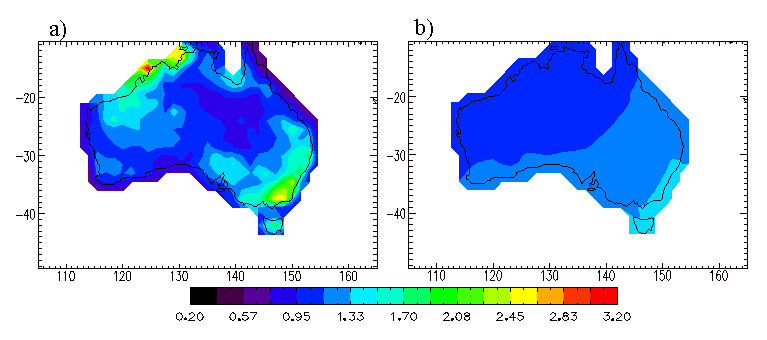
\includegraphics{Figures/Node_20_CoV-power}
\par\end{centering}

\caption{Node 20 Coefficient of Variance for a) wind power and b) DSR. \label{fig:Node20-CoV-Wind-Dsr}}
\end{figure}
 

As can be seen from Fig. \ref{fig:Node20-CoV-Wind-Dsr}, the standard
deviation of the DSR values for node 20 was always less than the mean
value, but for the wind power graph the same cannot be said. Particularly
for the high average wind power areas, the variability of wind power
values around that mean was quite large, indicating that the average
representation was less informative than hoped. To more clearly determine
how varied the wind and solar availability for node 20 was, the examination
of some extreme cases for node 20 was deemed necessary. 

Fig. \ref{fig:Node20-Lowest-Combined-Cap} depicts the occurrence
of node 20 that had the lowest combined wind and solar capacity during
the day. Daytime occurrences were only considered when finding the
lowest renewable capacity simply because the minimum in DSR at night
was not a feature of the synoptic regime for node 20. Fig. \ref{fig:Node20-Lowest-Combined-Cap}---when
a ridging high pressure system is centred east of Victoria---could
therefore be thought of as a worst case scenario for the large-scale
wind and solar resource availability of Australia. 
\begin{figure}[H]
\begin{centering}
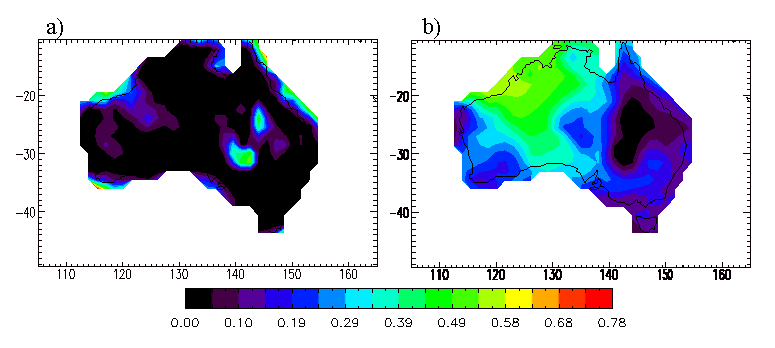
\includegraphics{Figures/Node_20_min_capacity-wind}
\par\end{centering}

\caption{a) Wind power capacity and b) DSR capacity for the occurrence of continental
SOM node 20 that leads to the lowest combined daytime capacity (0600UTC
May 15 1997). \label{fig:Node20-Lowest-Combined-Cap}}
\end{figure}


Fig. \ref{fig:Node20-Lowest-Combined-Cap} also demonstrates the type
of synoptic regime that perhaps cannot be planned for when designing
a large-scale renewable electricity network across Australia. However,
knowledge of the possibility of very low wind and solar availability
for the node 20 synoptic regime could also prove to be useful for
forecasting purposes. That is, the wind and solar conditions illustrated
in Fig. \ref{fig:Node20-Lowest-Combined-Cap} could serve as a first
guess for a forecast of the pressure distribution in Fig. \ref{fig:Node20-Min-day-Comp-MSLP}b.
Planning ahead of time for such low capacities would allow a more
sophisticated electricity system that incorporates other renewables,
storage options and back-ups to still meet the demand for electricity.
In reality, an electricity network would be designed to include such
back-ups and varied resources, rather than simply relying on wind
and solar PV power. To ensure that 0600UTC on May 15 1997 was indeed
an accurate occurrence of node 20 Fig. \ref{fig:Node20-Min-day-Comp-MSLP}
compares the pressure distributions of node 20 and 0600UTC on May
15 1997. 
\begin{figure}[H]
\begin{centering}
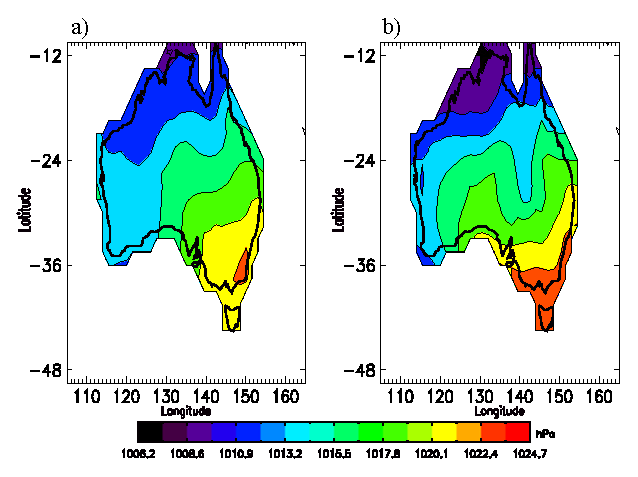
\includegraphics{Figures/SOM_comp_node20_min-cap}
\par\end{centering}

\caption{Comparison between the MSLP for a) continental SOM node 20 and b)
0600UTC May 15 1997. \label{fig:Node20-Min-day-Comp-MSLP}}
\end{figure}


The other extreme considered for node 20 was the occurrence that led
to the highest average capacity value for both wind power and DSR.
Somewhat expectedly, Fig. \ref{fig:Node20-Highest-Combined-Cap} suggests
that despite the low average capacity of both wind power and DSR for
node 20 and the potentially very poor output from Fig. \ref{fig:Node20-CoV-Wind-Dsr}
there were some daytime occurrences of node 20 that were favourable
for wind and solar availability. As can be seen from the pressure
distribution that gave rise to the wind and solar conditions in Fig.
\ref{fig:Node20-Highest-Combined-Cap} (Fig. \ref{fig:Node20-Max-day-Comp-MSLP})
a slight change in high pressure centre and intensity led to quite
different wind and solar conditions, in spite of the same SOM node
classification. 
\begin{figure}[H]
\begin{centering}
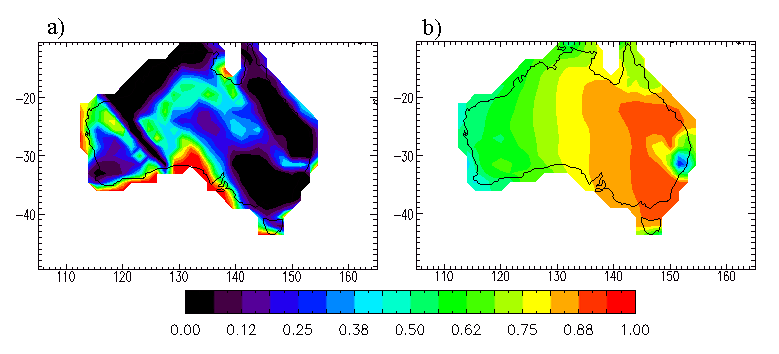
\includegraphics{Figures/Node_20_max_capacity-wind}
\par\end{centering}

\caption{a) Wind power capacity and b) DSR capacity for the occurrence of continental
SOM node 20 that led to the highest combined capacity (0000UTC November
24 1996). \label{fig:Node20-Highest-Combined-Cap}}
\end{figure}


An unfortunate consequence of the SOM technique, along with most other
data synthesis techniques, is the fact that the SOM nodes never occurr
exactly. Pressure distributions that were different but closely related
were said to belong to each SOM node, which then allowed for the quite
different wind and solar capacities (seen in Fig. \ref{fig:Node20-Lowest-Combined-Cap}
and Fig. \ref{fig:Node20-Highest-Combined-Cap}) to be assigned to
the same SOM node. The difference between Fig. \ref{fig:Node20-Lowest-Combined-Cap}
and Fig. \ref{fig:Node20-Highest-Combined-Cap} also serves as an
example of how varied the wind and solar fields can be from pressure
distributions that are similar (it could then be expected that the
same might also occur for other SOM nodes). This variance around a
given SOM node could be an argument for the use of wind speed and
solar irradiance SOMs, as these are the fields of interest. However,
the continuous nature of MSLP variability on synoptic scales makes
it much more amenable to a SOM than a field like wind speed (whose
variance would be much larger and therefore much harder to summarise
in a reasonable number of nodes). 
\begin{figure}[H]
\begin{centering}
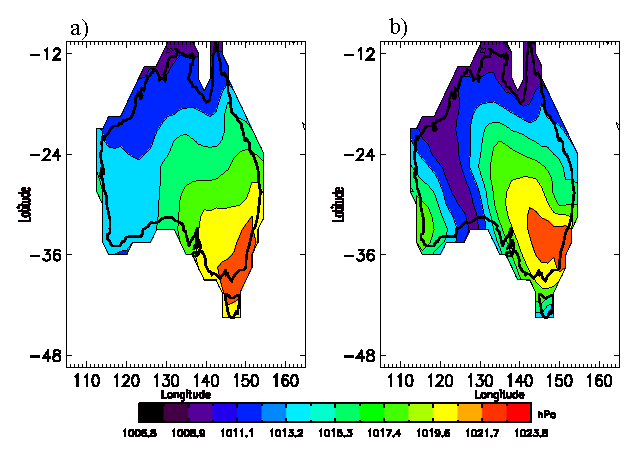
\includegraphics{Figures/SOM_comp_node20_max-cap}
\par\end{centering}

\caption{Comparison between the MSLP for a) continental SOM node 20 and b)
0000UTC November 24 1996. \label{fig:Node20-Max-day-Comp-MSLP}}
\end{figure}
 

The SOM node that averaged the highest combined wind and solar capacities,
node 24, had average wind power and DSR capacities described in Fig.
\ref{fig:Node24-Wind-Dsr-Cap}. On average, node 24 was characterised
by concurrently high wind and solar availability on the west coast
of WA. Node 24 provided another important example of the spatial relationship
between the wind and solar fields and was therefore also an important
node to study. 
\begin{figure}[H]
\begin{centering}
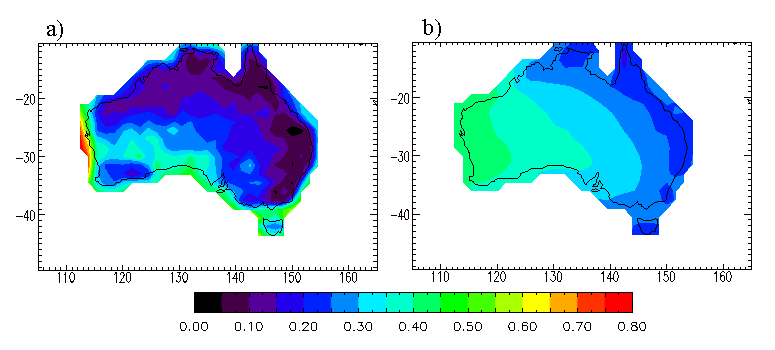
\includegraphics{Figures/Node_24_average_power-cap_wind_cap}
\par\end{centering}

\caption{Average capacity when continental SOM node 24 occurs for a) wind power
and b) DSR. \label{fig:Node24-Wind-Dsr-Cap}}
\end{figure}


Fig. \ref{fig:Node24-Highest-Combined-Cap} follows on from the earlier
analysis of node 20 by depicting the occurrence of node 24 that had
the highest combined wind power and DSR capacities. The pressure distribution
associated with the wind and solar capacities in Fig. \ref{fig:Node24-Highest-Combined-Cap}
(Fig. \ref{fig:Node24-Max-day-Comp-MSLP}b) indicates a fairly deep
high pressure system centred at about 125�E and 40�S, which is essentially
just a deeper version of node 24 (Fig. \ref{fig:Node24-Max-day-Comp-MSLP}a).
Onshore winds at the time of maximum wind and solar availability for
node 24 explain the generally higher wind power capacities seen in
Fig. \ref{fig:Node24-Highest-Combined-Cap}, however, it was interesting
to note that these maxima in South Australia were not very consistent
with the average map in Fig. \ref{fig:Node24-Wind-Dsr-Cap}. The maximum
average wind power capacity for node 24 was along the coast of WA,
but this location in Fig. \ref{fig:Node24-Highest-Combined-Cap} was
not an area of particularly high wind power capacity, and certainly
not in comparison with other areas. The DSR capacities for the best
case scenario of node 24 appeared to match the average map in a much
more consistent manner than the wind power capacity map---with the
exception of central Queensland and New South Wales. The minimum in
DSR for Fig. \ref{fig:Node24-Highest-Combined-Cap} was co-located
with the low pressure tendencies (perhaps the remnants of a tropical
low) seen in Fig. \ref{fig:Node24-Max-day-Comp-MSLP}, which could
indicate some convective behaviour and thus cloud cover. Meanwhile
the smaller pressure gradients near the low in Fig. \ref{fig:Node24-Max-day-Comp-MSLP}
could explain some of the low wind power tendencies associated with
the minimum in DSR.
\begin{figure}[H]
\begin{centering}
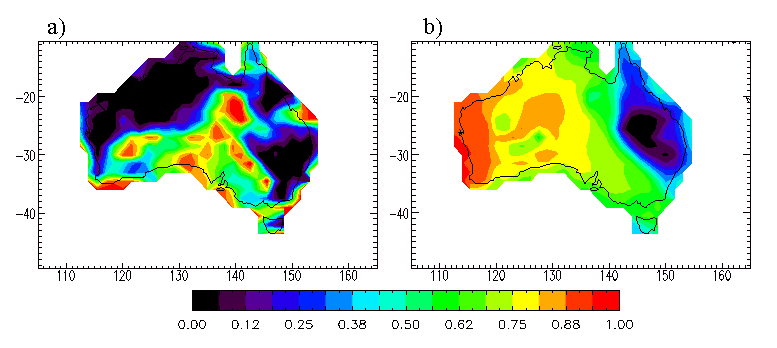
\includegraphics{Figures/Node_24_max_capacity-wind_field}
\par\end{centering}

\caption{a) Wind power capacity and b) DSR capacity for the occurrence of continental
SOM node 24 that leads to the highest combined capacity (0600UTC January
16 2008). \label{fig:Node24-Highest-Combined-Cap}}
\end{figure}
\begin{figure}[H]
\begin{centering}
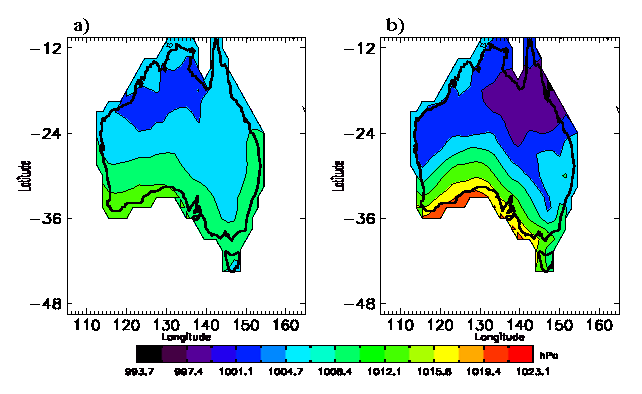
\includegraphics{Figures/SOM_comp_node24_max-cap}
\par\end{centering}

\caption{Comparison between the MSLP for a) continental SOM node 24 and b)
0600UTC January 16 2008. \label{fig:Node24-Max-day-Comp-MSLP}}
\end{figure}


In comparison to the analysis when node 24 produced the highest combined
wind and solar capacity, the occurrence of node 24 that led to the
lowest combined wind and solar capacity had a distribution of wind
and solar availability that was much more closely aligned with the
average map for node 24 (Fig. \ref{fig:Node24-Lowest-Combined-Cap}).
The maximum in Fig. \ref{fig:Node24-Lowest-Combined-Cap}a suggests
that despite there being maxima at other locations in Fig. \ref{fig:Node24-Highest-Combined-Cap}a,
high wind power capacities for the central coast of WA were a persistent
pattern for the majority of node 24 occurrences. For the central coast
of WA 89\% of node 24 occurrences had a peak wind power capacity value
greater than 0.7 and 79\% had an average wind power capacity value
of greater than 0.5; the central coast of WA was considered to be
the region of (112.5�E, 240S-28.5�S) and (114�E, 28.5�S-33�S), which
was the region of high wind power capacity in Fig. \ref{fig:Node24-Wind-Dsr-Cap}a.
Similar results were also obtained for the DSR capacity values, except
the persistence was even higher due to the smooth nature of the DSR
data. The fact that such a high percentage of occurrences for node
24 had high wind power capacity values (and DSR capacity values) in
the same region of WA was a key finding, which could also serve as
a forecasting guide in much the same manner as the low output occurrence
for node 20. 
\begin{figure}[H]
\begin{centering}
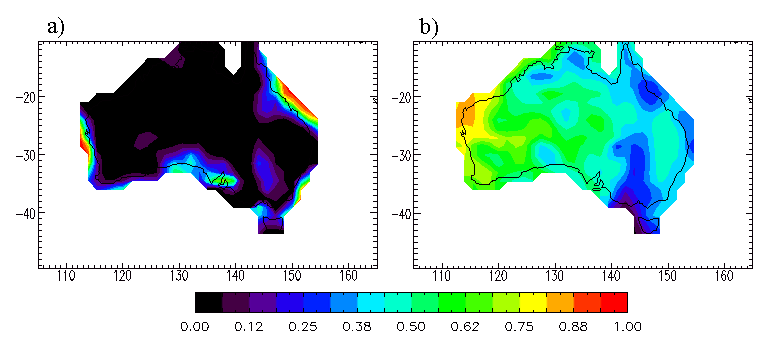
\includegraphics{Figures/Node_24_min_capacity-wind_field}
\par\end{centering}

\caption{a) Wind power capacity and b) DSR capacity for the occurrence of continental
SOM node 24 that leads to the lowest combined daytime capacity (0600UTC
March 15 2007). \label{fig:Node24-Lowest-Combined-Cap}}
\end{figure}


The pressure distribution that accompanied the wind and solar distributions
in Fig. \ref{fig:Node24-Lowest-Combined-Cap} were closely related
to node 24 (to be expected) (Fig. \ref{fig:Node24-Min-day-Comp-MSLP}),
but if the mean flow is predominantly west-east, also represented
an early/less evolved version of node 24. The more westerly centred
high pressure system for the best case scenario of node 24 allowed
for two high centres to be visible in the domain, which also allowed
for a trough to be present in between at about 140�E. The suggestion
of a trough at 140�E was consistent with the minimum in DSR capacity
seen in Fig. \ref{fig:Node24-Lowest-Combined-Cap}b and perhaps also
the higher wind power capacity values in the wake of the trough (Fig.
\ref{fig:Node24-Lowest-Combined-Cap}a). 
\begin{figure}[H]
\begin{centering}
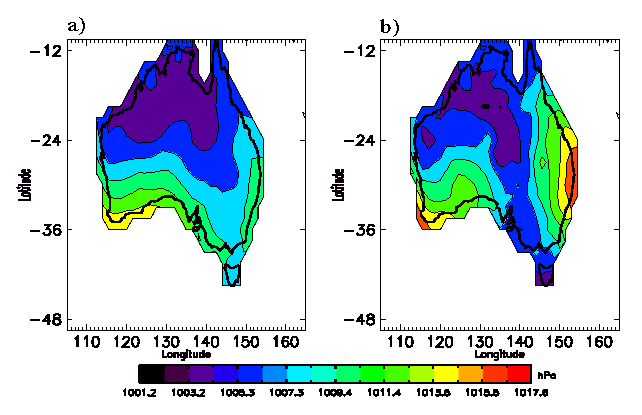
\includegraphics{Figures/SOM_comp_node24_min-cap}
\par\end{centering}

\caption{Comparison between the MSLP for a) continental SOM node 24 and b)
0600UTC March 15 2007. \label{fig:Node24-Min-day-Comp-MSLP}}
\end{figure}


Both nodes 20 and 24 have proven useful in terms of their representation
of co-located and concurrent wind and solar minima or maxima, however,
node 18 could also be seen as useful because it had maxima in the
wind and solar fields that were not co-located (Fig. \ref{fig:Node18-Wind-Dsr-Cap}).
Although the maxima for node 18 did not contain capacity values as
high as the maxima for node 24, node 18 did have the most prominent
maxima that were not co-located. 
\begin{figure}[H]
\begin{centering}
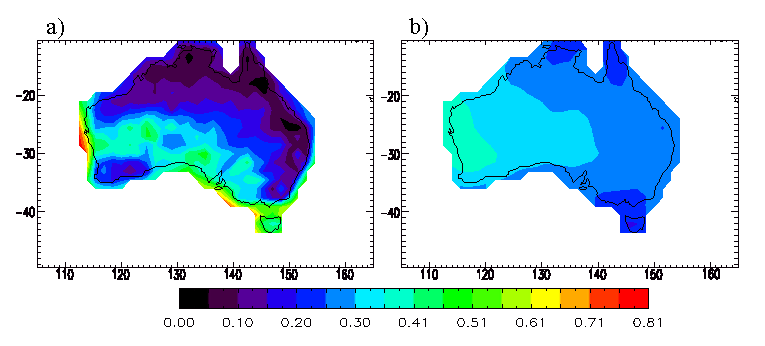
\includegraphics{Figures/Node_18_average_dsr_wind-cap}
\par\end{centering}

\caption{Average capacity when continental SOM node 18 occurs for a) wind power
and b) DSR. \label{fig:Node18-Wind-Dsr-Cap}}
\end{figure}


The regions identified as maxima for node 18 were in south-western
Victoria (wind power capacity) and the central coast of WA (DSR capacity).
In order to investigate the extremes for node 18 it was necessary
to formally define these two regions such that identification of when
the combined capacity from the two regions was either at its lowest
or highest was possible. Fig. \ref{fig:Node18-High-Regions} describes
the boundaries of the two maxima regions, which were then used in
a similar manner to the previous analyses of node 20 and 24. 
\begin{figure}[H]
\begin{centering}
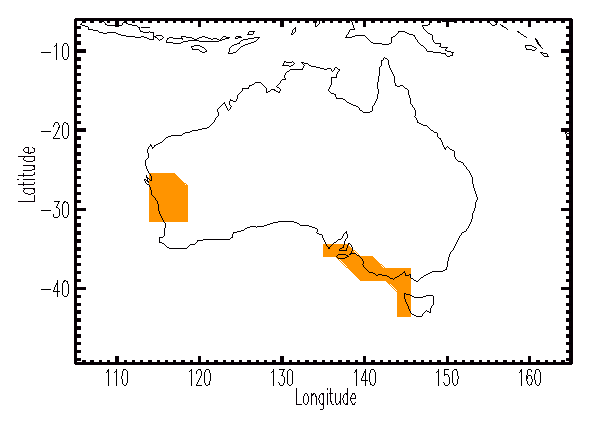
\includegraphics{Figures/Node_18_high_renew}
\par\end{centering}

\caption{The two regions identified as having separate average wind power and
DSR capacity maxima for node 18. The region in WA is the DSR maximum
and the region in the south is the wind power maximum. \label{fig:Node18-High-Regions}}
\end{figure}


The occurrence of node 18 that led to the highest combined capacity
of the two regions from Fig. \ref{fig:Node18-High-Regions} has wind
power and DSR capacities depicted in Fig. \ref{fig:Node18-High-Cap-Regions}.
As can be seen from Fig. \ref{fig:Node18-High-Cap-Regions}, and true
to the average map, the best case scenario for node 18 has a large
area of high wind power capacity through South Australia, Victoria
and Tasmania, as well as an extended region of high DSR capacity in
WA. The MSLP map that led to the best case scenario for node 18 indicates
a deep low pressure system centred just east of Tasmania (Fig. \ref{fig:Node18-Max-day-Comp-MSLP}).
The passage of the low pressure system accounted for the high wind
power capacities in southern Australia, while the offshore winds from
the high centred south of WA explained the higher DSR capacities.
\begin{figure}[H]
\begin{centering}
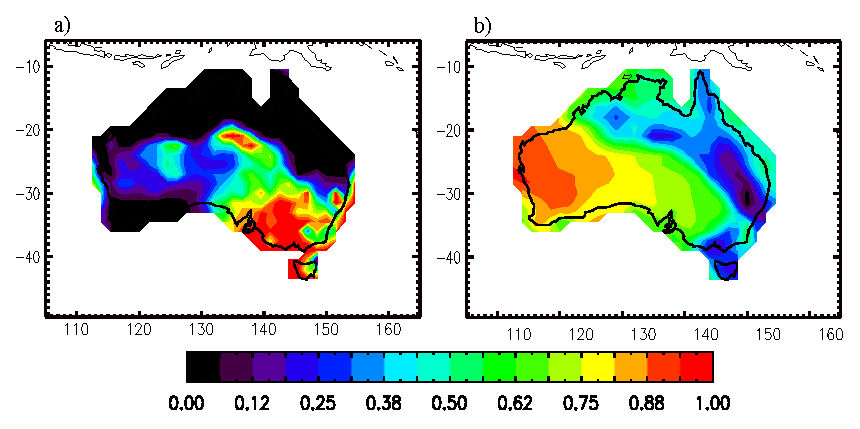
\includegraphics{Figures/Node_18_max_capacity-wind}
\par\end{centering}

\caption{a) Wind power capacity and b) DSR capacity for the occurrence of continental
SOM node 18 that leads to the highest combined capacity for the two
regions identified in Fig. \ref{fig:Node18-High-Regions} (0600UTC
December 22 2007). \label{fig:Node18-High-Cap-Regions}}
\end{figure}
\begin{figure}[H]
\begin{centering}
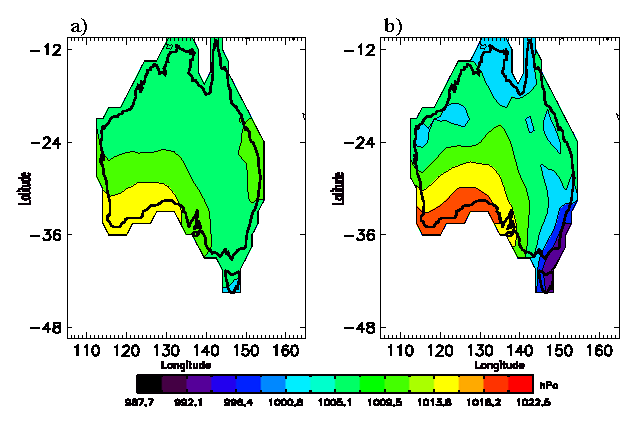
\includegraphics{Figures/SOM_comp_node18_max-cap}
\par\end{centering}

\caption{Comparison between the MSLP for a) continental SOM node 18 and b)
0600UTC December 22 2007. \label{fig:Node18-Max-day-Comp-MSLP}}
\end{figure}


However, and as was seen for the other nodes, a slight change in the
longitude of the high pressure system that characterises node 18 led
to a vastly different distribution of wind power and DSR capacity
values (Fig. \ref{fig:Node18-Lowest-Combined-Cap-Regions} and Fig.
\ref{fig:Node18-Min-day-Comp-MSLP}). The minimum combined capacity
for node 18 had virtually no wind capacity in the area of southern
Australia identified in Fig. \ref{fig:Node18-High-Regions} and maxima
in DSR capacity away from the area of high DSR capacity identified
in Fig. \ref{fig:Node18-High-Regions}. Yet, based on Fig. \ref{fig:Node18-Min-day-Comp-MSLP},
it was easy to see why 0000UTC on March 3 1999 was still classified
as an occurrence of node 18. The fact that the eventual wind power
and DSR capacity distributions were so dependent on the particular
longitude and strength of the high pressure systems added a qualification
to the use of the SOM nodes as forecasting tool. That is, for a MSLP
forecast that is said to match a SOM node, one must consider the quality
of the SOM node match before using the wind power and DSR capacity
maps as a first guess of the wind and solar availability of the Australian
region.
\begin{figure}[H]
\begin{centering}
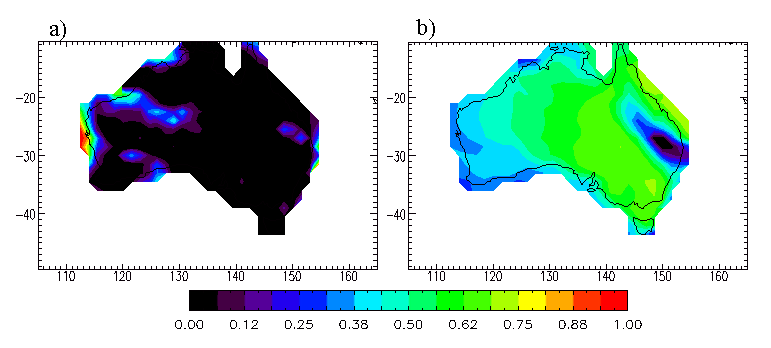
\includegraphics{Figures/Node_18_min_capacity-wind}
\par\end{centering}

\caption{a) Wind power capacity and b) DSR capacity for the occurrence of continental
SOM node 18 that leads to the lowest combined daytime capacity for
the two regions identified in Fig. \ref{fig:Node18-High-Regions}
(0000UTC March 3 1999). \label{fig:Node18-Lowest-Combined-Cap-Regions}}
\end{figure}
\begin{figure}[H]
\begin{centering}
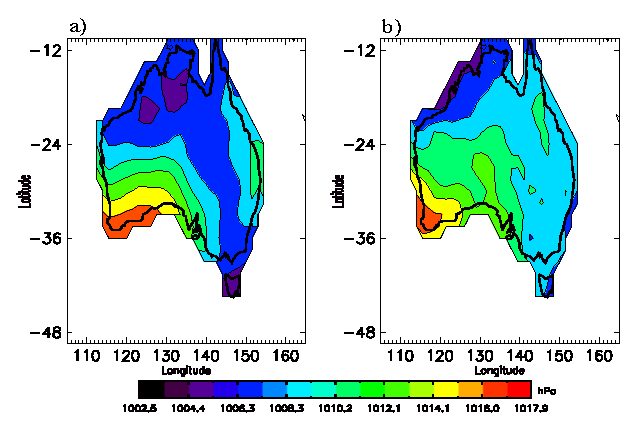
\includegraphics{Figures/SOM_comp_node18_min-cap}
\par\end{centering}

\caption{Comparison between the MSLP for a) continental SOM node 18 and b)
0000UTC March 3 1999. \label{fig:Node18-Min-day-Comp-MSLP}}
\end{figure}
 

The analysis of some of the SOM nodes that appeared either favourable
or detrimental for the simultaneous wind and solar electricity production
of the Australian region highlighted an important aspect of the variability
of the wind and solar fields that was independent of the SOM classification
process. That despite the advantages of the SOM technique it will
seemingly always be possible to have time steps that pass the BMU
filtering process, which are then classed as belonging to the same
SOM node, but whose MSLP distributions lead to very different wind
power and DSR capacity distributions for the Australian region. 

The SOM node analysis also highlighted some potentially advantageous
persistent features of the wind and, to a lesser extent, solar fields.
For instance, the summertime higher wind power capacity values along
the coast of WA appeared in even the worst case scenario for nodes
18 and 24. The SOM analysis therefore identified the central coast
of WA as a particularly good wind resource. However, publicly available
figures suggest this wind resource is yet to be utilised---only one
wind farm of significant size has been built in this area of the WA
coast (89MW Alinta wind farm, near Geraldton; \citealp{Council2012a}.),
presumably due to a lack of population to service in the immediate
area. 


\subsection{Time of Day Biases in SOM Node Occurrences\label{sub:SOM-Cont-Time-of-Day}}

A final but important consideration for the SOM analysis, particularly
for the DSR analysis, could be any time of day biases in the occurrence
of the SOM nodes. If, for instance, there was a bias towards the afternoon
occurrence of a particular node then it would be expected that artificially
inflated DSR values, which are not necessarily a reflection of the
synoptic conditions for that node, would occur. Fig. \ref{fig:Time-of-Day-SOM-Occ}
shows the percentage occurrence of each SOM node and for each time
of day, in order to investigate the time-of-day tendencies of the
SOM nodes from Fig. \ref{fig:6x5-SOM-space-Cont}. The statistical
significance of the SOM node occurrences in Fig. \ref{fig:Time-of-Day-SOM-Occ}
was assessed using a Monte-Carlo approach. 10,000 time-series of randomly
assigned numbers from 1-30 were created and then the statistics for
each SOM number calculated based on the number of times the SOM node
was said to occur at 0000UTC (the first time step), 0600UTC (the second
time step), 1200UTC (the third time step), 1800UTC (the fourth time
step) and so on for each time step in each of the randomly generated
time series. 99\% confidence that a percentage occurrence could not
be due to random processes was then calculated based on the top 50
(unusually high) and bottom 50 (unusually low) occurrences, out of
the 10,000.
\begin{figure}[H]
\begin{centering}
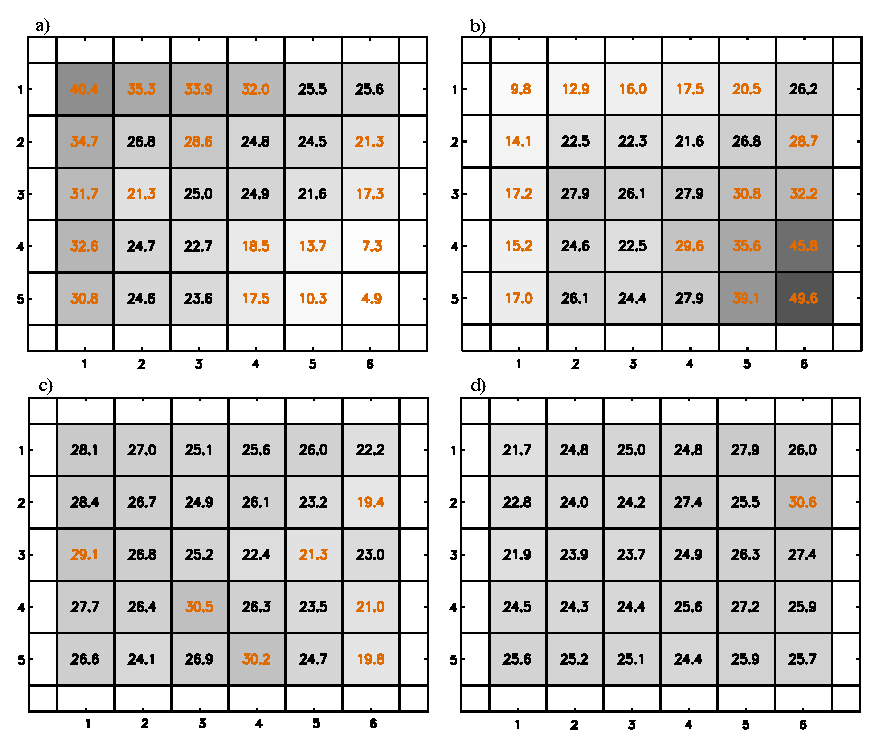
\includegraphics{Figures/time-of-day_SOM_cont_filtered_00-18UTC}
\par\end{centering}

\caption{The percentage occurrence of each continental SOM node (Fig. \ref{fig:6x5-SOM-space-Cont})
at a) 0000UTC, b) 0600UTC, c) 1200UTC and d) 1800UTC. Numbers in orange
represent significant values using a two-tailed Monte-Carlo simulation
at the one percent confidence range and darker grey indicates larger
values. \label{fig:Time-of-Day-SOM-Occ}}
\end{figure}
 

As can be seen from Fig. \ref{fig:Time-of-Day-SOM-Occ}, there were
indeed some nodes that had a significantly high or low occurrence
at a particular time of day. SOM node 30, for instance, had almost
half of its occurrences at 0600UTC, and then only 5\% at 0000UTC.
There also appeared to be division in the SOM space such that the
nodes that occurred significantly more often at 0000UTC occurred significantly
less often at 0600UTC, and vice versa. With reference to Fig. \ref{fig:SOM-Cont-Surf-Seasnl-Occ}
the nodes that occurred most often at 0000UTC in Fig. \ref{fig:Time-of-Day-SOM-Occ}
were also the so-called winter-only nodes and the nodes that occurred
most often at 0600UTC were the so-called summer-only nodes. It is
most likely that such biases in the occurrence rate of some of the
SOM nodes was due, at least in part, by atmospheric tides. 

\citet{Dai1999} in their study of diurnal and semi-diurnal tides
in the global surface pressure fields succinctly summarised the process
of atmospheric tides by saying that \textquotedblleft{}atmospheric
solar heating, combined with upward eddy conduction of heat from the
ground, generates gravity waves in the atmosphere at periods of the
integral fractions of the solar day\textquotedblright{} and that \textquotedblleft{}these
waves cause regular oscillations in atmospheric wind, temperature,
and pressure fields, which are often referred to as atmospheric tides\textquotedblright{}.
\citet{Dai1999} also demonstrated that the diurnal wave in the surface
pressure field is dominated by continental upward sensible heat flux;
a finding that appears to be supported by the earlier work of \citet{Kong1995},
which examined diurnal surface pressure variations over the Australian
continent. 

In terms of the biases seen in Fig. \ref{fig:Time-of-Day-SOM-Occ},
the winter nodes that appeared most commonly at 0000UTC (10am in the
East, 8am in the West) seemed to match the peak in the diurnal-wave
amplitude (high pressure anomalies) suggested by \citet{Dai1999}
as these nodes were dominated by higher pressure, particularly at
higher latitudes. The reverse could be said for the summer nodes that
appeared most often at 0600UTC (5pm in the East, 2pm in the West).
The summer-nodes were in agreement with the minimum in the diurnal-wave
amplitude (lower pressure over much of the continent \citet{Dai1999})
and the maximum in the upwards sensible heat flux (diurnal heating
that was a maximum in the afternoon and also in summer). The atmospheric
tide theory does not suggest that a high will become a low depending
on the time of day, which is unphysical, but it does give a physical
reason for why there might be a higher probability of the winter nodes
that were said to occur most often in the morning and the summer nodes
that were said to occur most often in the afternoon, were classed
as occurring more often in the morning and afternoon. The probability
of SOM node 30 occurring in the afternoon was elevated due to an upwards
sensible heat flux, which was then reversed in the morning and gives
rise to the reduced probability of SOM node 30 occurring at that time. 


\section{Decorrelation Analysis}

In this section the ERA-Interim data were analysed for how well, or
not, the data were correlated with each other. The term decorrelation
relates to the distance at which two points in the domain have a significantly
different time series to be considered unrelated. The length at which
such a decorrelation occurs could, in particular for the wind field,
indicate inherent features of the synoptic scale variability over
Australia (i.e. the width of a high pressure system). Such information
could be exploited in the design of a large-scale renewable electricity
network for Australia and thus deserves further investigation. Here,
certain locations were correlated with the rest of the domain and
then statistical significance was obtained for each correlation value
in the domain. A type of Monte-Carlo simulation, described in \citet{Ebisuzaki1997},
was utilised to determine the significance of a correlation for a
given significance level. The \citet{Ebisuzaki1997} method was utilised
because of the auto-correlation that exists in the wind field, which
is not conserved in the normal Monte-Carlo approach of reordering
time steps. In this section, however, only the wind field was considered.
The representation of DSR in ERA-Interim, even at three-hourly intervals,
was too smooth to obtain significantly different time series anywhere
in the continental domain (not shown). For instance, a lot of the
variability introduced by clouds and aerosols is not resolved at 3-hourly
averaged values and at \textasciitilde{}166km spatial resolution.
Instead, the solar variability captured by ERA-Interim is heavily
influenced by diurnal and seasonal cycles, which do not vary enough
across the continent to result in uncorrelated time series.


\subsection{Method}

Counter to the common approach to a Monte-Carlo simulation, which
involves the random reordering of data points in a time series, the
method described in \citet{Ebisuzaki1997} involves the random reordering
of phases in a time series. By means of a Fourier transform, and then
reverse Fourier transform, the \citet{Ebisuzaki1997} method is able
to conserve the autocorrelation of a time series. Conservation of
the autocorrelation is an important aspect of the \citet{Ebisuzaki1997}
method; not only because this is not guaranteed with the traditional
Monte-Carlo method but also because the autocorrelation of a time
series is a defining feature of most meteorological fields. Commonly,
the approach for dealing with autocorrelated data is to sub-sample
the time series every few data points, depending on the level of autocorrelation.
The sub-sampling allows the user to include only data that are independent
of the previous time step. The process of sub-sampling, however, also
reduces the degrees of freedom in the time series, which can affect
later statistical testing. This thesis does not utilise the sub-sampling
process but instead employs the \citet{Ebisuzaki1997} method to create
many versions of a time series with the same level of autocorrelation,
and then the versions are used for testing statistical significance. 

The relatively coarse temporal and spatial resolution of the ERA-Interim
data means that the wind and solar fields that the current study utilises
tend to be quite smooth. Thus these fields commonly exhibit autocorrelations
that do not reach near zero values for lags less than three or four
time steps. The mathematical interpretation of the \citet{Ebisuzaki1997}
method is described in the following three steps, taken from the paper. 
\begin{itemize}
\item Step 1: Compute the discrete Fourier transform of the first series,
$a_{j}$, by
\end{itemize}
\begin{equation}
a_{k}=\frac{2-\delta_{k}}{N}\overset{N-1}{\underset{j=0}{\sum}}a_{j}e^{\frac{2\pi ijk}{N}},\label{eq:Ebisuzaki-Step-1}
\end{equation}


where $\delta_{k}=0$ except for $k=0,\frac{N}{2}$ (even $N$) in
which case $\delta_{k}=1$.
\begin{itemize}
\item Step 2: Let $r_{0}=0$, $r_{k}=\mid a_{k}\mid exp(i\theta_{k})$ for
$0<k<\frac{N}{2}$, and $r_{\frac{N}{2}}=\sqrt{2}\mid a_{\frac{N}{2}}\mid cos(\theta_{\frac{N}{2}})$
for even $N$, where $\theta_{k}$ is a uniform variable from $[0,2\pi)$.
\item Step 3: Compute the inverse Fourier transform of $r_{k}$ by
\end{itemize}
\begin{equation}
r_{j}=\mathbb{R}\overset{n}{\underset{k=0}{\sum}}r_{k}e^{\frac{-2\pi ijk}{N}},\label{eq:Ebisuzaki-Step-3}
\end{equation}


where $n=\frac{N}{2}$ or $\frac{N-1}{2}$ for even and odd $N$,
respectively.

In the three steps described above the original series $a_{j}$ is
divided into its Fourier components, whose phase is then randomised
by $\theta_{k}$. The result, $r_{j}$, which has the same dimensionality
as the original series, is simply the inverse Fourier transform of
steps 1 and 2. Steps 1-3 can then be repeated with different $\theta_{k}$
to produce multiple versions of the original series, storing the resultant
$r_{j}$ to use for statistical significance calculations.


\subsection{Results and Discussion}

Fig. \ref{fig:Decorrel-Point-Correlation-Cities} shows maps of point
correlations of the 80m wind speed where the points were chosen based
on major population centres (the likely location of renewable electricity
infrastructure) and where the stippling indicates areas of either
negative correlation or locations that are considered significantly
different. Statistical significance is calculated based on a 10,000
member bootstrap of the \citet{Ebisuzaki1997} method outlined above.
Correlations between the cities and everywhere else were calculated
for each randomised version of the wind speed at each city in Fig.
\ref{fig:Decorrel-Point-Correlation-Cities}. A correlation was said
to be significantly close to zero at the 5\% confidence level if it
was less than the 500th member of the absolute value of the collection
of correlations at each grid-point. Negative correlations or correlations
that were significantly close to zero were the measures of whether
or not two locations had 80m wind speed time series that were unrelated,
or alternatively anticorrelated. 
\begin{figure}[H]
\begin{centering}
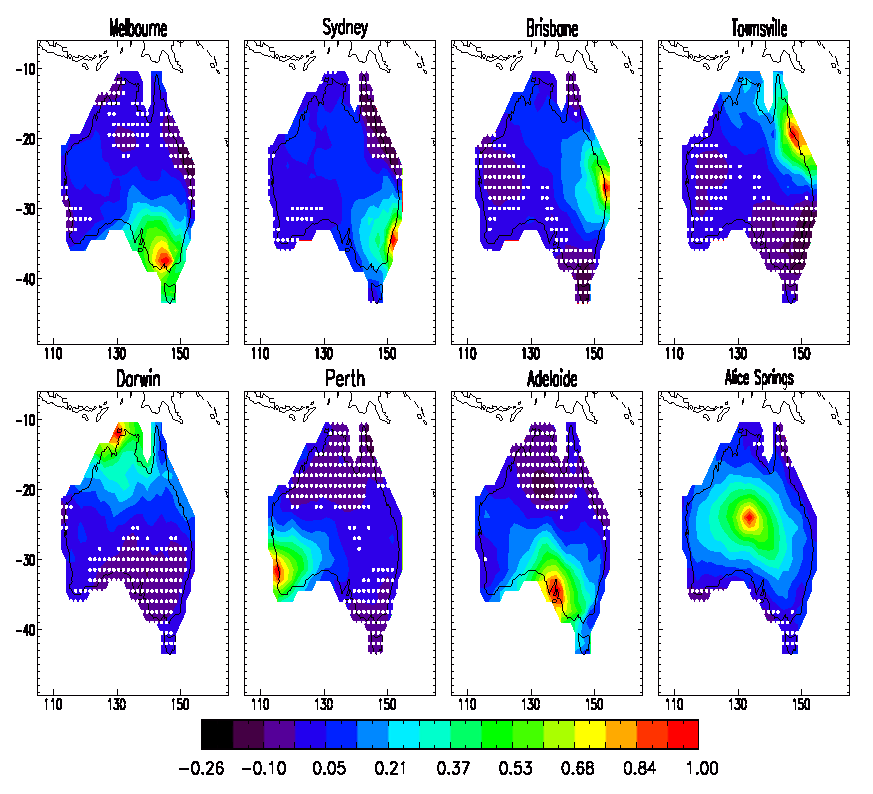
\includegraphics{Figures/Ebisuzaki_all-cities}
\par\end{centering}

\caption{Point correlation maps for some of the major population centres across
the Australian continent. Stippling indicates areas of negative correlation
or where the correlation is statistically different to the population
centre using the \citet{Ebisuzaki1997} method. \label{fig:Decorrel-Point-Correlation-Cities}}
\end{figure}


When considering the net power output from two locations that have
statistically different wind speed time series it is easy to see how
the information contained in Fig. \ref{fig:Decorrel-Point-Correlation-Cities}
is important for any large-scale connection of wind power across the
Australian continent. According to Fig. \ref{fig:Decorrel-Point-Correlation-Cities}
the average distance at which the wind field first becomes statistically
different appears to be roughly 1,300km-1,400km. Therefore, two wind
installations on the Australian continent separated by about 1,400km
are likely to have unrelated wind speed time series. This, of course,
does not guarantee opposing output, which would require a correlation
of -1, but it does give an estimate for the distance at which a significant
advantage could be gained when considering the separation of wind
power resources across Australia. Both the steadiness of the net output
and the price of electricity produced by the separated wind installations
could be maximised when considering the decorrelation distances suggested
by Fig. \ref{fig:Decorrel-Point-Correlation-Cities}. That is, assuming
wind installations that are part of the same electricity market, a
higher price of electricity could be sought if one of the installations
is able to produce electricity when the other cannot and therefore
when there is also a higher demand for electricity in the market. 


\section{Conclusion\label{sec:Cov-Conclusion}}

This chapter examined aspects of the covariance of the wind and solar
fields from ERA-Interim by categorising the weather of the Australian
region into SOM nodes and analysing the wind and solar conditions
that co-occurred with the regimes. Node 20 (high pressure centred
east of Victoria) was identified as being associated with low capacity
of both wind and solar, node 24 (high pressure centred well south
of Perth) associated with co-located high capacity of wind and solar,
and node 18 (high pressure centred just south of Perth) as being associated
with dispersed areas of high wind and solar capacity. It was found
that while these nodes were on average low/high capacity nodes---with
some examples of very high/low output---they were not exclusively
high/low weather systems. Rather, there was a varied association,
centred about a high/low average, between weather system and wind
and solar potential.

Time-of-day biases in the occurrence of the SOM nodes were also examined.
It was found that there was an elevated chance of certain nodes occurring
at specific times of day based on atmospheric tide theory, but this
was seen as unlikely to dictate that a particular node was favourable/poor
for solar capacity as it was the diurnal variations in solar output
over the continent largely driving the tides in the first place.

Finally, the \citet{Ebisuzaki1997} method for correlating two time
series of varying autocorrelation was utilised with the 80m wind speed
data to identify a decorrelation length scale in the wind field. Using
point correlations as examples, rather than a matrix of cross-correlations,
it was found that the average separation needed for two locations
to lose their significant association was on the order of 1,300-1,400km.
Although it should be noted that this length could be dependent on
the temporal resolution of the data (six-hourly for ERA-Interim).
Higher resolution data might result in a smaller length due to the
variance missed by the current six-hourly resolution.

In the next part to this thesis the covariance of wind and solar is
further explored via an optimised electricity system. For the majority
of Part 2 the focus is on just the eastern states of Australia (the
National Electricity Network (NEM) region), as opposed to the whole
country. The two parts of the thesis are linked in later chapters
and the difference in domain size (whole country versus NEM) is noted.
Part 1 necessitates that a large domain encompassing the whole country
be used in order to capture the synoptic scale. However, Part 2 explores
in detail the variability only over the NEM region because this is
the likely location for future wind and solar capacities. The influence
of the larger synoptic scale systems on the NEM-wide variability in
wind and solar is then analysed.
\end{document}
